\chapter{Die Benutzeroberfl�che}
Im Vergleich zur �lteren XChat Version, m�chte ich hier nur die Ver�nderungen
erw�hnen, die gegen�ber der �lteren Version gemacht wurden. Au�erdem ist
anzumerken, dass sich die �bersetzung in die eigene Landessprache noch in der
Entwicklung befindet. Die Einzelnen hier angesprochenen Teile der
Benutzeroberfl�che kann man ein- und ausblenden, indem man das Kontextmen�
durch klicken mit der Rechten Maustaste im Textfenster aufruft.

\section{Die Men�zeile}\index{XChat 2 !Men�zeile}

\begin{figure}[htb]
  \begin{center}
    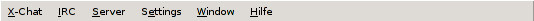
\includegraphics[width=6.0in]{xchat2_images/menubar.png}
  \end{center}
  \caption{Ansicht der Men�zeile}
  \label{fig:menuezeile2}
\end{figure}

Die Men�zeile wurde gegen�ber der alten Version etwas aufger�umt. So befinden
sich folgende Men�punkte in der Men�zeile:
\begin{description}
  \item[Server List] Verwalten der IRC Server und Netzwerke mit denen man in
  Verbindung treten kann. Au�erdem k�nnen noch Verbindungsoptionen
  eingestellt werden.
  
  \item[New] �ber die Untermen�s, kann man neue Server- und Kanalreiter, sowie
  Fenster zum Hauptfenster des XChat hinzuf�gen.
  
  \item[Load Plugin or Script\dots] Neue Plugins oder Skripte k�nnen �ber
  diesen Men�punkt zum XChat hinzugeladen werden. XChat kann mit Perl-, Tcl-
  und Pythonscripts erweitert werden. Abh�ngig ist dies jedoch von der
  Distribution und der Kompilation des Programms.
 
  \item[Detach Tab] Hier kann der aktuelle Reiter aus dem Hauptfenster ``abgetrennt''
  werden. Der Reiter erscheint dann in einem neuen Fenster.
  
  \item[Close Tab] Der aktuelle Reiter kann mit diesem Men�punkt geschlossen werden.
  \item[Beenden] Hiermit kann XChat beendet werden.
\end{description}


\section{Die Toolzeile}\index{XChat 2 !Toolzeile}
Die Toolzeile hat sich gegen�ber der alten Version kaum ver�ndert. Die
Funktion $\rightarrow$ \emph{Detach Tab} ist in die Men�zeile mit
eingegliedert worden. Mehr �ber die Men�zeile gibt es auf Seite
\pageref{sec:toolzeile}.

\begin{figure}[htb]
  \begin{center}
    
\includegraphics[width=6.0in]{xchat2_images/toolbar.png}
  \end{center}
  \caption{Ansicht der Toolbar}
  \label{fig:toolbar2}
\end{figure}


\section{Das Textfenster}\index{XChat 2 !Textfenster}
Das Textfenster erf�llt wie in der alten Version des XChat das anzeigen des
Textes (wer h�tte das wohl gedacht ;-)). Mehr dazu auf Seite
\pageref{sec:textfenster}.

\begin{figure}[htb]
  \begin{center}
    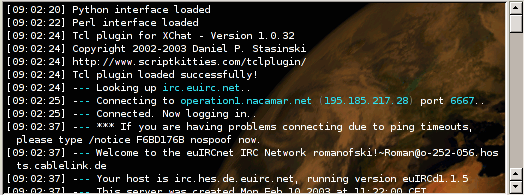
\includegraphics[width=6.0in]{xchat2_images/textbox.png}
  \end{center}
  \caption{Ansicht des Textfensters}
  \label{fig:textfenster2}
\end{figure}

\section{Die Benutzerliste}
Im Vergleich zur alten Version des XChat, kann man nun per Maus die
Benutzerliste aus der rechten Seite herausziehen und dort wieder
hineinschieben.
Die Funktionalit�t der Benutzerliste ist aber gleich geblieben.

\begin{figure}[htb]
  \begin{center}
    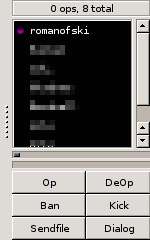
\includegraphics[width=1.5in]{xchat2_images/userlist.png}
  \end{center}
  \caption{Benutzerliste}
  \label{fig:benutzerliste2}
\end{figure}


\section{Die Eingabezeile}\index{XChat 2 !Eingabezeile}
Die Eingabezeile wurde in seiner Funktionalit�t etwas abge�ndert. So kann man
den Nick f�r den aktuellen Reiter durch klicken auf dessen �ndern. Durch
klicken auf die Eingabezeile mit der rechten Maustaste, kann man zus�tzlich noch
\begin{itemize}
  \item Text ausschneiden, kopieren, einf�gen und alles markieren
  \item die Eingabemethode �ndern und
  \item Unicode-Steuerzeichen einf�gen
\end{itemize}

\section{Reiter oder Tabs}

\section{Server List}
